\section{概览}
本文的背景技术分析部分介绍了当前的动态分析相关技术和实现工具以及Android系统的部分运行原理\juhao 结合前面的分析和系统实现的可行性, 本系统整体实现方案如下:

采用\ref{artInstr}节提到的ART Instrumentation的技术, 修改Android8.1系统源代码中ART虚拟机部分来实现Java层次的方法调用监控和简单的脱壳功能\juhao 通过Frida工具来实现对本地函数调用以及Java层特定方法的监控, 同时增加监控系统的灵活性和可扩展性\juhao 修改Android源代码中与应用启动相关的部分实现监控应用的启动情况, 在目标应用启动时开启其他监控功能\juhao 通过简化日志内容和使用内存缓存日志的方式实现更为高效的日志系统用于保存监控系统记录的数据\juhao 通过系统属性来实现目标应用和其他配置选项的设置\juhao 

图\ref{emOverview}描述了系统的总体设计, 加粗的矩形部分为本系统的模块\juhao 其中EvMonitor-core模块运行在ART内部, 负责监控Java方法调用, dex文件解析, 并且实现了日志系统\juhao 该部分还通过JNI给运行在应用层的EvMonitor-startLogger模块提供了接口, 可以启动和关闭监控功能, 调用日志系统等, 这些接口也通过导出函数的方式提供给EvMonitor-Frida调用\juhao EvMonitor-Frida是一个本地动态链接库, 用于实现对本地层函数调用以及某些特别感兴趣的Java层方法的监控, 在目标应用进程加载应用文件之前被加载到目标进程中, 开启对目标应用的监控\juhao 
\begin{figure}[ht]
	\centering
	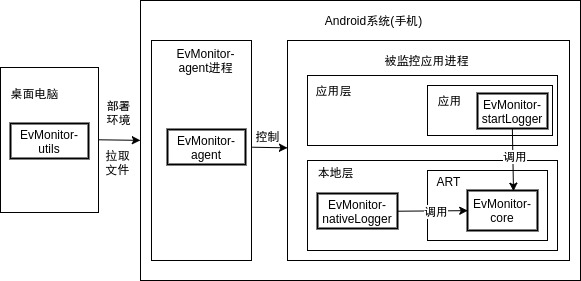
\includegraphics[width=\textwidth]{em_overview.jpg}
	\caption{EvMonitor概览}
	\label{emOverview}
\end{figure}

\section{监控应用启动}
本功能由EvMonitor-startLogger实现\juhao 
\ref{appStartA}节详细介绍了Android系统应用的启动过程\juhao 由于Android应用进程不是通过直接使用应用APK文件启动, 而是通过Zygote进程fork产生, 因此无法按照传统PC上启动子进程, 然后加载监控模块开启监控, 最后再加载目标应用开始执行的方式来实现在应用加载前启动对应用的监控\juhao 只有通过监控应用的启动, 在能够获取到应用的名称并且应用自身代码还未执行时开启完成监控应用的初始化操作\juhao ActivityThread类的handleBindApplication方法开始的位置符合上述条件, 因此本系统选择在handleBindApplication方法的适当位置添加监控代码\juhao 

监控代码的实现逻辑如图所示\juhao
首先读取当前进程名和应用名(有些应用会启动多个进程), 使用日志系统记录当前启动的应用名和进程名\juhao 接着读取系统属性em.target\_type, 确定是只监控某个进程还是监控该应用的全部进程\juhao 接着根据上述结果读取系统属性获取要监控的进程名或者应用名并同本进程或者应用名比较, 如果不同则退出监控代码, 不启动监控系统; 如果相同则调用Evmonitor-core提供的初始化监控的接口来启动对该应用的监控\juhao 之后再根据当前运行环境是32位还是64位加载对应的EvMonitor-Frida动态链接库, 完成监控系统的初始化\juhao 

为了便于调用JNI和被调用, 我将上述监控代码作为一个新的静态方法加入了com.android.internal.os.Zygote类中, 并通过在Zygote类中增加本地方法的方式调用了EvMonitor-core提供的本地层接口\juhao 

\section{Java方法调用监控}
本功能由EvMonitor-core实现\juhao 
为了能够获取到应用所有Java方法调用行为, 本系统选择在ART内执行方法的函数中加入监控代码\juhao  \ref{methodExecA}节详细介绍了ART虚拟机执行方法的过程\juhao 根据分析, 在ArtMethod::Invoke和Execute函数中插入监控代码就能够记录所有的Java方法调用情况\juhao  

\section{本地函数调用监控}
本功能由EvMonitor-Frida实现\juhao 本系统使用Frida工具的动态链接库形式(frida-gadget), 通过在应用加载自身代码之前加载frida-gadget并执行监控代码来实现对本地层函数调用的监控\juhao 

\section{脱壳功能}
本功能由EvMonitor-core实现\juhao 
目前Android平台应用加固工具的加壳机制十分复杂, 本系统根据\ref{classLoadA}节介绍的类加载过程, 选取了用于dex文件加载的关键函数即位于安卓源代码中/art/runtime/DexFile.cc中DexFile类的构造函数DexFile()来实现简单脱壳获取dex文件的功能\juhao 

\section{日志系统}
本功能由EvMonitor-core实现\juhao 
